% Options for packages loaded elsewhere
\PassOptionsToPackage{unicode}{hyperref}
\PassOptionsToPackage{hyphens}{url}
%
\documentclass[
]{article}
\title{Econometrie II : Transports}
\usepackage{etoolbox}
\makeatletter
\providecommand{\subtitle}[1]{% add subtitle to \maketitle
  \apptocmd{\@title}{\par {\large #1 \par}}{}{}
}
\makeatother
\subtitle{Rapport}
\author{Guewen HESLAN - Bijan VALILOU}
\date{Janvier 2021}

\usepackage{amsmath,amssymb}
\usepackage{lmodern}
\usepackage{iftex}
\ifPDFTeX
  \usepackage[T1]{fontenc}
  \usepackage[utf8]{inputenc}
  \usepackage{textcomp} % provide euro and other symbols
\else % if luatex or xetex
  \usepackage{unicode-math}
  \defaultfontfeatures{Scale=MatchLowercase}
  \defaultfontfeatures[\rmfamily]{Ligatures=TeX,Scale=1}
\fi
% Use upquote if available, for straight quotes in verbatim environments
\IfFileExists{upquote.sty}{\usepackage{upquote}}{}
\IfFileExists{microtype.sty}{% use microtype if available
  \usepackage[]{microtype}
  \UseMicrotypeSet[protrusion]{basicmath} % disable protrusion for tt fonts
}{}
\makeatletter
\@ifundefined{KOMAClassName}{% if non-KOMA class
  \IfFileExists{parskip.sty}{%
    \usepackage{parskip}
  }{% else
    \setlength{\parindent}{0pt}
    \setlength{\parskip}{6pt plus 2pt minus 1pt}}
}{% if KOMA class
  \KOMAoptions{parskip=half}}
\makeatother
\usepackage{xcolor}
\IfFileExists{xurl.sty}{\usepackage{xurl}}{} % add URL line breaks if available
\IfFileExists{bookmark.sty}{\usepackage{bookmark}}{\usepackage{hyperref}}
\hypersetup{
  pdftitle={Econometrie II : Transports},
  pdfauthor={Guewen HESLAN - Bijan VALILOU},
  hidelinks,
  pdfcreator={LaTeX via pandoc}}
\urlstyle{same} % disable monospaced font for URLs
\usepackage[margin=1in]{geometry}
\usepackage{color}
\usepackage{fancyvrb}
\newcommand{\VerbBar}{|}
\newcommand{\VERB}{\Verb[commandchars=\\\{\}]}
\DefineVerbatimEnvironment{Highlighting}{Verbatim}{commandchars=\\\{\}}
% Add ',fontsize=\small' for more characters per line
\usepackage{framed}
\definecolor{shadecolor}{RGB}{248,248,248}
\newenvironment{Shaded}{\begin{snugshade}}{\end{snugshade}}
\newcommand{\AlertTok}[1]{\textcolor[rgb]{0.94,0.16,0.16}{#1}}
\newcommand{\AnnotationTok}[1]{\textcolor[rgb]{0.56,0.35,0.01}{\textbf{\textit{#1}}}}
\newcommand{\AttributeTok}[1]{\textcolor[rgb]{0.77,0.63,0.00}{#1}}
\newcommand{\BaseNTok}[1]{\textcolor[rgb]{0.00,0.00,0.81}{#1}}
\newcommand{\BuiltInTok}[1]{#1}
\newcommand{\CharTok}[1]{\textcolor[rgb]{0.31,0.60,0.02}{#1}}
\newcommand{\CommentTok}[1]{\textcolor[rgb]{0.56,0.35,0.01}{\textit{#1}}}
\newcommand{\CommentVarTok}[1]{\textcolor[rgb]{0.56,0.35,0.01}{\textbf{\textit{#1}}}}
\newcommand{\ConstantTok}[1]{\textcolor[rgb]{0.00,0.00,0.00}{#1}}
\newcommand{\ControlFlowTok}[1]{\textcolor[rgb]{0.13,0.29,0.53}{\textbf{#1}}}
\newcommand{\DataTypeTok}[1]{\textcolor[rgb]{0.13,0.29,0.53}{#1}}
\newcommand{\DecValTok}[1]{\textcolor[rgb]{0.00,0.00,0.81}{#1}}
\newcommand{\DocumentationTok}[1]{\textcolor[rgb]{0.56,0.35,0.01}{\textbf{\textit{#1}}}}
\newcommand{\ErrorTok}[1]{\textcolor[rgb]{0.64,0.00,0.00}{\textbf{#1}}}
\newcommand{\ExtensionTok}[1]{#1}
\newcommand{\FloatTok}[1]{\textcolor[rgb]{0.00,0.00,0.81}{#1}}
\newcommand{\FunctionTok}[1]{\textcolor[rgb]{0.00,0.00,0.00}{#1}}
\newcommand{\ImportTok}[1]{#1}
\newcommand{\InformationTok}[1]{\textcolor[rgb]{0.56,0.35,0.01}{\textbf{\textit{#1}}}}
\newcommand{\KeywordTok}[1]{\textcolor[rgb]{0.13,0.29,0.53}{\textbf{#1}}}
\newcommand{\NormalTok}[1]{#1}
\newcommand{\OperatorTok}[1]{\textcolor[rgb]{0.81,0.36,0.00}{\textbf{#1}}}
\newcommand{\OtherTok}[1]{\textcolor[rgb]{0.56,0.35,0.01}{#1}}
\newcommand{\PreprocessorTok}[1]{\textcolor[rgb]{0.56,0.35,0.01}{\textit{#1}}}
\newcommand{\RegionMarkerTok}[1]{#1}
\newcommand{\SpecialCharTok}[1]{\textcolor[rgb]{0.00,0.00,0.00}{#1}}
\newcommand{\SpecialStringTok}[1]{\textcolor[rgb]{0.31,0.60,0.02}{#1}}
\newcommand{\StringTok}[1]{\textcolor[rgb]{0.31,0.60,0.02}{#1}}
\newcommand{\VariableTok}[1]{\textcolor[rgb]{0.00,0.00,0.00}{#1}}
\newcommand{\VerbatimStringTok}[1]{\textcolor[rgb]{0.31,0.60,0.02}{#1}}
\newcommand{\WarningTok}[1]{\textcolor[rgb]{0.56,0.35,0.01}{\textbf{\textit{#1}}}}
\usepackage{longtable,booktabs,array}
\usepackage{calc} % for calculating minipage widths
% Correct order of tables after \paragraph or \subparagraph
\usepackage{etoolbox}
\makeatletter
\patchcmd\longtable{\par}{\if@noskipsec\mbox{}\fi\par}{}{}
\makeatother
% Allow footnotes in longtable head/foot
\IfFileExists{footnotehyper.sty}{\usepackage{footnotehyper}}{\usepackage{footnote}}
\makesavenoteenv{longtable}
\usepackage{graphicx}
\makeatletter
\def\maxwidth{\ifdim\Gin@nat@width>\linewidth\linewidth\else\Gin@nat@width\fi}
\def\maxheight{\ifdim\Gin@nat@height>\textheight\textheight\else\Gin@nat@height\fi}
\makeatother
% Scale images if necessary, so that they will not overflow the page
% margins by default, and it is still possible to overwrite the defaults
% using explicit options in \includegraphics[width, height, ...]{}
\setkeys{Gin}{width=\maxwidth,height=\maxheight,keepaspectratio}
% Set default figure placement to htbp
\makeatletter
\def\fps@figure{htbp}
\makeatother
\setlength{\emergencystretch}{3em} % prevent overfull lines
\providecommand{\tightlist}{%
  \setlength{\itemsep}{0pt}\setlength{\parskip}{0pt}}
\setcounter{secnumdepth}{5}
\usepackage{fancyhdr}
\pagestyle{fancy}
\fancyfoot[CO,CE]{Econométrie II}
\fancyfoot[LE,RO]{\thepage}
\usepackage{booktabs}
\usepackage{longtable}
\usepackage{array}
\usepackage{multirow}
\usepackage{wrapfig}
\usepackage{float}
\usepackage{colortbl}
\usepackage{pdflscape}
\usepackage{tabu}
\usepackage{threeparttable}
\usepackage{threeparttablex}
\usepackage[normalem]{ulem}
\usepackage{makecell}
\usepackage{xcolor}
\ifLuaTeX
  \usepackage{selnolig}  % disable illegal ligatures
\fi
\usepackage[]{biblatex}
\addbibresource{references.bib}

\begin{document}
\maketitle

{
\setcounter{tocdepth}{2}
\tableofcontents
}
\newpage

\hypertarget{introduction}{%
\section{Introduction}\label{introduction}}

\begin{Shaded}
\begin{Highlighting}[]
\FunctionTok{library}\NormalTok{(usethis)}
\FunctionTok{library}\NormalTok{(readxl)}
\FunctionTok{library}\NormalTok{(gitcreds)}
\FunctionTok{library}\NormalTok{(strucchange)}
\end{Highlighting}
\end{Shaded}

\begin{verbatim}
## Le chargement a nécessité le package : zoo
\end{verbatim}

\begin{verbatim}
## 
## Attachement du package : 'zoo'
\end{verbatim}

\begin{verbatim}
## Les objets suivants sont masqués depuis 'package:base':
## 
##     as.Date, as.Date.numeric
\end{verbatim}

\begin{verbatim}
## Le chargement a nécessité le package : sandwich
\end{verbatim}

\begin{Shaded}
\begin{Highlighting}[]
\FunctionTok{library}\NormalTok{(gets)}
\end{Highlighting}
\end{Shaded}

\begin{verbatim}
## Le chargement a nécessité le package : parallel
\end{verbatim}

\begin{Shaded}
\begin{Highlighting}[]
\FunctionTok{library}\NormalTok{(ggplot2)}
\FunctionTok{library}\NormalTok{(kableExtra)}
\FunctionTok{library}\NormalTok{(pander)}
\end{Highlighting}
\end{Shaded}

\begin{Shaded}
\begin{Highlighting}[]
\NormalTok{Transport\_France2019 }\OtherTok{\textless{}{-}} \FunctionTok{read\_excel}\NormalTok{(}\StringTok{"Transport\_France2019\_v2.xlsx"}\NormalTok{)}

\DocumentationTok{\#\#Vecteurs des séries}
\CommentTok{\#Qtt\_Trsp\_route \textless{}{-} Transport\_France2019$Qtt\_Trsp\_route}
\CommentTok{\#Qtt\_Trsp\_train \textless{}{-} Transport\_France2019$Qtt\_Trsp\_train}
\CommentTok{\#Pdiesel \textless{}{-} Transport\_France2019$Pdiesel}
\CommentTok{\#Qdiesel \textless{}{-} Transport\_France2019$QDiesel}
\CommentTok{\#GDP \textless{}{-} Transport\_France2019$GDP}
\CommentTok{\#CPI \textless{}{-} Transport\_France2019$CPI}
\CommentTok{\#QDieselCamion \textless{}{-} Transport\_France2019$Qdieselcamion}
\end{Highlighting}
\end{Shaded}

\begin{Shaded}
\begin{Highlighting}[]
\DocumentationTok{\#\#Séries temporelles}
\NormalTok{Qtt\_Trsp\_route.ts }\OtherTok{\textless{}{-}} \FunctionTok{ts}\NormalTok{(Transport\_France2019}\SpecialCharTok{$}\NormalTok{Qtt\_Trsp\_route, }\AttributeTok{start=}\FunctionTok{c}\NormalTok{(}\DecValTok{1985}\NormalTok{) , }\AttributeTok{end=}\FunctionTok{c}\NormalTok{(}\DecValTok{2019}\NormalTok{), }\AttributeTok{frequency=}\DecValTok{1}\NormalTok{)}
\NormalTok{Qtt\_Trsp\_train.ts }\OtherTok{\textless{}{-}} \FunctionTok{ts}\NormalTok{(Transport\_France2019}\SpecialCharTok{$}\NormalTok{Qtt\_Trsp\_train, }\AttributeTok{start=}\FunctionTok{c}\NormalTok{(}\DecValTok{1985}\NormalTok{) , }\AttributeTok{end=}\FunctionTok{c}\NormalTok{(}\DecValTok{2019}\NormalTok{), }\AttributeTok{frequency=}\DecValTok{1}\NormalTok{)}
\NormalTok{Pdiesel.ts }\OtherTok{\textless{}{-}} \FunctionTok{ts}\NormalTok{(Transport\_France2019}\SpecialCharTok{$}\NormalTok{Pdiesel, }\AttributeTok{start=}\FunctionTok{c}\NormalTok{(}\DecValTok{1985}\NormalTok{) , }\AttributeTok{end=}\FunctionTok{c}\NormalTok{(}\DecValTok{2019}\NormalTok{), }\AttributeTok{frequency=}\DecValTok{1}\NormalTok{)}
\NormalTok{Qdiesel.ts }\OtherTok{\textless{}{-}} \FunctionTok{ts}\NormalTok{(Transport\_France2019}\SpecialCharTok{$}\NormalTok{QDiesel, }\AttributeTok{start=}\FunctionTok{c}\NormalTok{(}\DecValTok{1985}\NormalTok{) , }\AttributeTok{end=}\FunctionTok{c}\NormalTok{(}\DecValTok{2019}\NormalTok{), }\AttributeTok{frequency=}\DecValTok{1}\NormalTok{)}
\NormalTok{GDP.ts }\OtherTok{\textless{}{-}} \FunctionTok{ts}\NormalTok{(Transport\_France2019}\SpecialCharTok{$}\StringTok{"PIB en volume (en milliards d\textquotesingle{}euros 2014)"}\NormalTok{, }\AttributeTok{start=}\FunctionTok{c}\NormalTok{(}\DecValTok{1985}\NormalTok{) , }\AttributeTok{end=}\FunctionTok{c}\NormalTok{(}\DecValTok{2019}\NormalTok{), }\AttributeTok{frequency=}\DecValTok{1}\NormalTok{)}
\NormalTok{CPI.ts }\OtherTok{\textless{}{-}} \FunctionTok{ts}\NormalTok{(Transport\_France2019}\SpecialCharTok{$}\NormalTok{CPI, }\AttributeTok{start=}\FunctionTok{c}\NormalTok{(}\DecValTok{1985}\NormalTok{) , }\AttributeTok{end=}\FunctionTok{c}\NormalTok{(}\DecValTok{2019}\NormalTok{), }\AttributeTok{frequency=}\DecValTok{1}\NormalTok{)}
\NormalTok{Qdieselcamion.ts }\OtherTok{\textless{}{-}} \FunctionTok{ts}\NormalTok{(Transport\_France2019}\SpecialCharTok{$}\NormalTok{Qdieselcamion, }\AttributeTok{start=}\FunctionTok{c}\NormalTok{(}\DecValTok{1985}\NormalTok{) , }\AttributeTok{end=}\FunctionTok{c}\NormalTok{(}\DecValTok{2019}\NormalTok{), }\AttributeTok{frequency=}\DecValTok{1}\NormalTok{)}
\end{Highlighting}
\end{Shaded}

\begin{Shaded}
\begin{Highlighting}[]
\DocumentationTok{\#\#Graph en niveau}
\FunctionTok{ggplot}\NormalTok{() }\SpecialCharTok{+} 
  \FunctionTok{geom\_line}\NormalTok{( }\FunctionTok{aes}\NormalTok{(}\AttributeTok{x =}\NormalTok{ Transport\_France2019}\SpecialCharTok{$}\NormalTok{Year,}\AttributeTok{y =}\NormalTok{ Transport\_France2019}\SpecialCharTok{$}\NormalTok{Qtt\_Trsp\_route))}\SpecialCharTok{+}
\FunctionTok{labs}\NormalTok{(}\AttributeTok{x =} \StringTok{"Année"}\NormalTok{, }\AttributeTok{y =} \StringTok{"Quantités transportées par route"}\NormalTok{, }\AttributeTok{title =} \StringTok{"Fig. X Quantités transportées par route"}\NormalTok{) }\SpecialCharTok{+} 
    \FunctionTok{theme}\NormalTok{(}\AttributeTok{axis.text=}\FunctionTok{element\_text}\NormalTok{(}\AttributeTok{size=}\DecValTok{6}\NormalTok{),}\AttributeTok{legend.text=}\FunctionTok{element\_text}\NormalTok{(}\AttributeTok{size=}\DecValTok{7}\NormalTok{),}\AttributeTok{axis.title=}\FunctionTok{element\_text}\NormalTok{(}\AttributeTok{size=}\DecValTok{9}\NormalTok{),}\AttributeTok{title =} \FunctionTok{element\_text}\NormalTok{(}\AttributeTok{size=}\DecValTok{9}\NormalTok{), }\AttributeTok{plot.title =} \FunctionTok{element\_text}\NormalTok{(}\AttributeTok{hjust =} \FloatTok{0.5}\NormalTok{, }\AttributeTok{vjust =} \FloatTok{0.5}\NormalTok{)) }\SpecialCharTok{+}
  \FunctionTok{scale\_x\_continuous}\NormalTok{(}\AttributeTok{breaks=}\FunctionTok{seq}\NormalTok{(}\DecValTok{1985}\NormalTok{,}\DecValTok{2019}\NormalTok{,}\DecValTok{5}\NormalTok{))}
\end{Highlighting}
\end{Shaded}

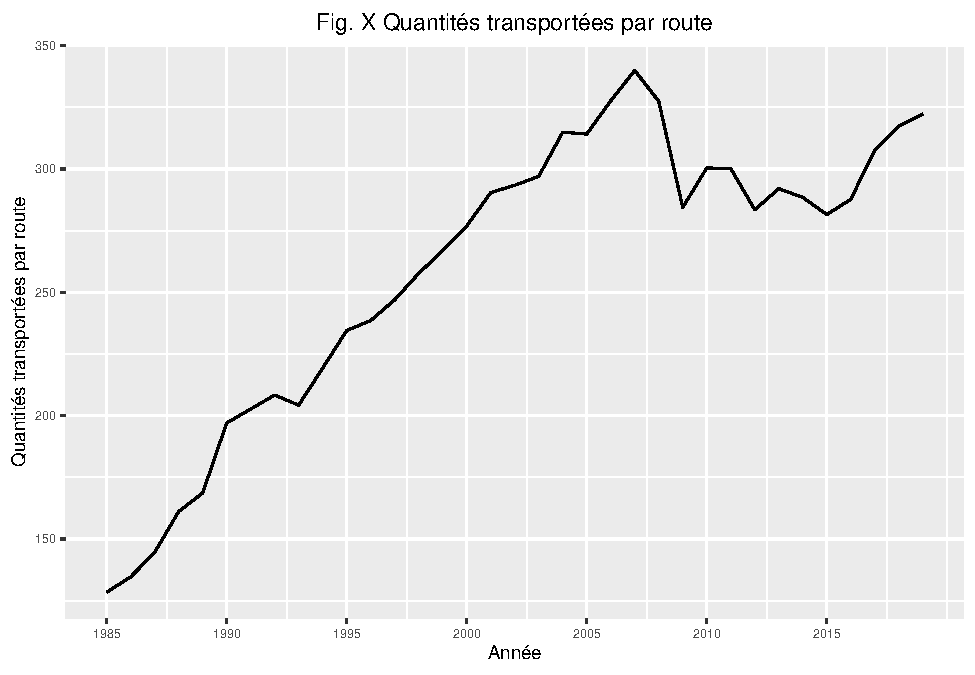
\includegraphics{Projet_econometrie_II_files/figure-latex/unnamed-chunk-4-1.pdf}

\begin{Shaded}
\begin{Highlighting}[]
\FunctionTok{ggplot}\NormalTok{() }\SpecialCharTok{+} 
  \FunctionTok{geom\_line}\NormalTok{( }\FunctionTok{aes}\NormalTok{(}\AttributeTok{x =}\NormalTok{ Transport\_France2019}\SpecialCharTok{$}\NormalTok{Year,}\AttributeTok{y =}\NormalTok{ Transport\_France2019}\SpecialCharTok{$}\NormalTok{Qtt\_Trsp\_train))}\SpecialCharTok{+}
\FunctionTok{labs}\NormalTok{(}\AttributeTok{x =} \StringTok{"Année"}\NormalTok{, }\AttributeTok{y =} \StringTok{"Quantités transportées par train"}\NormalTok{, }\AttributeTok{title =} \StringTok{"Fig. X Quantités transportées par train"}\NormalTok{) }\SpecialCharTok{+} 
    \FunctionTok{theme}\NormalTok{(}\AttributeTok{axis.text=}\FunctionTok{element\_text}\NormalTok{(}\AttributeTok{size=}\DecValTok{6}\NormalTok{),}\AttributeTok{legend.text=}\FunctionTok{element\_text}\NormalTok{(}\AttributeTok{size=}\DecValTok{7}\NormalTok{),}\AttributeTok{axis.title=}\FunctionTok{element\_text}\NormalTok{(}\AttributeTok{size=}\DecValTok{9}\NormalTok{),}\AttributeTok{title =} \FunctionTok{element\_text}\NormalTok{(}\AttributeTok{size=}\DecValTok{9}\NormalTok{), }\AttributeTok{plot.title =} \FunctionTok{element\_text}\NormalTok{(}\AttributeTok{hjust =} \FloatTok{0.5}\NormalTok{, }\AttributeTok{vjust =} \FloatTok{0.5}\NormalTok{)) }\SpecialCharTok{+}
  \FunctionTok{scale\_x\_continuous}\NormalTok{(}\AttributeTok{breaks=}\FunctionTok{seq}\NormalTok{(}\DecValTok{1985}\NormalTok{,}\DecValTok{2019}\NormalTok{,}\DecValTok{5}\NormalTok{))}
\end{Highlighting}
\end{Shaded}

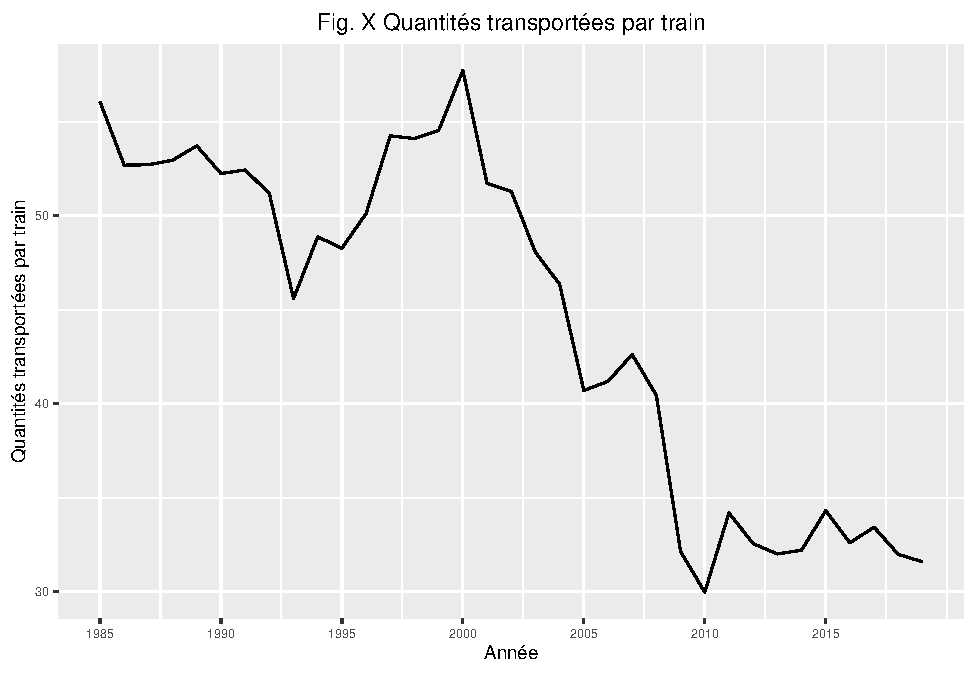
\includegraphics{Projet_econometrie_II_files/figure-latex/unnamed-chunk-4-2.pdf}

\begin{Shaded}
\begin{Highlighting}[]
\FunctionTok{ggplot}\NormalTok{() }\SpecialCharTok{+} 
  \FunctionTok{geom\_line}\NormalTok{( }\FunctionTok{aes}\NormalTok{(}\AttributeTok{x =}\NormalTok{ Transport\_France2019}\SpecialCharTok{$}\NormalTok{Year,}\AttributeTok{y =}\NormalTok{ Transport\_France2019}\SpecialCharTok{$}\NormalTok{Pdiesel))}\SpecialCharTok{+}
\FunctionTok{labs}\NormalTok{(}\AttributeTok{x =} \StringTok{"Année"}\NormalTok{, }\AttributeTok{y =} \StringTok{"Prix du disel"}\NormalTok{, }\AttributeTok{title =} \StringTok{"Fig. X Prix du diesel"}\NormalTok{) }\SpecialCharTok{+} 
    \FunctionTok{theme}\NormalTok{(}\AttributeTok{axis.text=}\FunctionTok{element\_text}\NormalTok{(}\AttributeTok{size=}\DecValTok{6}\NormalTok{),}\AttributeTok{legend.text=}\FunctionTok{element\_text}\NormalTok{(}\AttributeTok{size=}\DecValTok{7}\NormalTok{),}\AttributeTok{axis.title=}\FunctionTok{element\_text}\NormalTok{(}\AttributeTok{size=}\DecValTok{9}\NormalTok{),}\AttributeTok{title =} \FunctionTok{element\_text}\NormalTok{(}\AttributeTok{size=}\DecValTok{9}\NormalTok{), }\AttributeTok{plot.title =} \FunctionTok{element\_text}\NormalTok{(}\AttributeTok{hjust =} \FloatTok{0.5}\NormalTok{, }\AttributeTok{vjust =} \FloatTok{0.5}\NormalTok{)) }\SpecialCharTok{+}
  \FunctionTok{scale\_x\_continuous}\NormalTok{(}\AttributeTok{breaks=}\FunctionTok{seq}\NormalTok{(}\DecValTok{1985}\NormalTok{,}\DecValTok{2019}\NormalTok{,}\DecValTok{5}\NormalTok{))}
\end{Highlighting}
\end{Shaded}

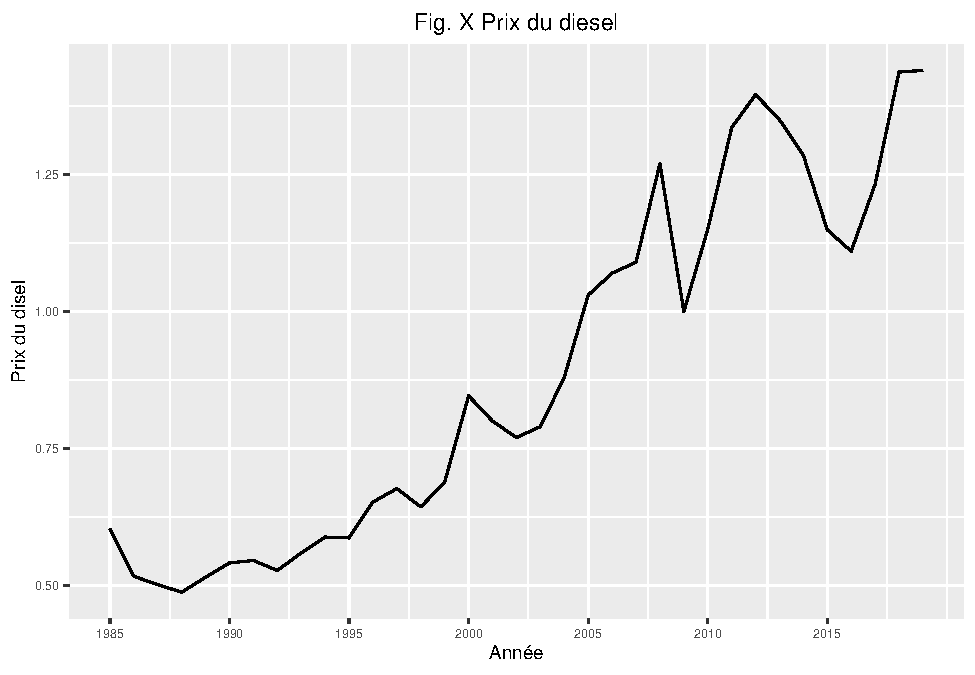
\includegraphics{Projet_econometrie_II_files/figure-latex/unnamed-chunk-4-3.pdf}

\begin{Shaded}
\begin{Highlighting}[]
\FunctionTok{ggplot}\NormalTok{() }\SpecialCharTok{+} 
  \FunctionTok{geom\_line}\NormalTok{( }\FunctionTok{aes}\NormalTok{(}\AttributeTok{x =}\NormalTok{ Transport\_France2019}\SpecialCharTok{$}\NormalTok{Year,}\AttributeTok{y =}\NormalTok{ Transport\_France2019}\SpecialCharTok{$}\StringTok{"PIB en volume (en milliards d\textquotesingle{}euros 2014)"}\NormalTok{))}\SpecialCharTok{+}
\FunctionTok{labs}\NormalTok{(}\AttributeTok{x =} \StringTok{"Année"}\NormalTok{, }\AttributeTok{y =} \StringTok{"PIB en volume (en milliards d\textquotesingle{}euros 2014)"}\NormalTok{, }\AttributeTok{title =} \StringTok{"Fig. X Produit intérieur brut"}\NormalTok{) }\SpecialCharTok{+} 
    \FunctionTok{theme}\NormalTok{(}\AttributeTok{axis.text=}\FunctionTok{element\_text}\NormalTok{(}\AttributeTok{size=}\DecValTok{6}\NormalTok{),}\AttributeTok{legend.text=}\FunctionTok{element\_text}\NormalTok{(}\AttributeTok{size=}\DecValTok{7}\NormalTok{),}\AttributeTok{axis.title=}\FunctionTok{element\_text}\NormalTok{(}\AttributeTok{size=}\DecValTok{9}\NormalTok{),}\AttributeTok{title =} \FunctionTok{element\_text}\NormalTok{(}\AttributeTok{size=}\DecValTok{9}\NormalTok{), }\AttributeTok{plot.title =} \FunctionTok{element\_text}\NormalTok{(}\AttributeTok{hjust =} \FloatTok{0.5}\NormalTok{, }\AttributeTok{vjust =} \FloatTok{0.5}\NormalTok{)) }\SpecialCharTok{+}
  \FunctionTok{scale\_x\_continuous}\NormalTok{(}\AttributeTok{breaks=}\FunctionTok{seq}\NormalTok{(}\DecValTok{1985}\NormalTok{,}\DecValTok{2019}\NormalTok{,}\DecValTok{5}\NormalTok{))}
\end{Highlighting}
\end{Shaded}

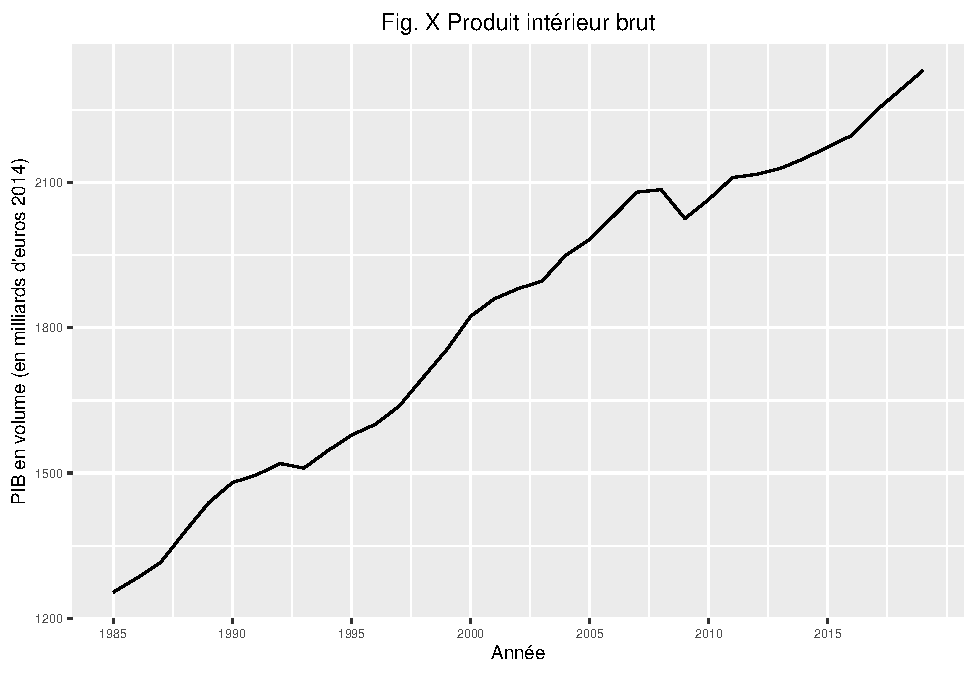
\includegraphics{Projet_econometrie_II_files/figure-latex/unnamed-chunk-4-4.pdf}

\begin{Shaded}
\begin{Highlighting}[]
\FunctionTok{ggplot}\NormalTok{() }\SpecialCharTok{+} 
  \FunctionTok{geom\_line}\NormalTok{( }\FunctionTok{aes}\NormalTok{(}\AttributeTok{x =}\NormalTok{ Transport\_France2019}\SpecialCharTok{$}\NormalTok{Year,}\AttributeTok{y =}\NormalTok{ Transport\_France2019}\SpecialCharTok{$}\StringTok{"PIB en volume (en milliards d\textquotesingle{}euros 2014)"}\NormalTok{))}\SpecialCharTok{+}
\FunctionTok{labs}\NormalTok{(}\AttributeTok{x =} \StringTok{"Année"}\NormalTok{, }\AttributeTok{y =} \StringTok{"PIB en volume (en milliards d\textquotesingle{}euros 2014)"}\NormalTok{, }\AttributeTok{title =} \StringTok{"Fig. X Produit intérieur brut"}\NormalTok{) }\SpecialCharTok{+} 
    \FunctionTok{theme}\NormalTok{(}\AttributeTok{axis.text=}\FunctionTok{element\_text}\NormalTok{(}\AttributeTok{size=}\DecValTok{6}\NormalTok{),}\AttributeTok{legend.text=}\FunctionTok{element\_text}\NormalTok{(}\AttributeTok{size=}\DecValTok{7}\NormalTok{),}\AttributeTok{axis.title=}\FunctionTok{element\_text}\NormalTok{(}\AttributeTok{size=}\DecValTok{9}\NormalTok{),}\AttributeTok{title =} \FunctionTok{element\_text}\NormalTok{(}\AttributeTok{size=}\DecValTok{9}\NormalTok{), }\AttributeTok{plot.title =} \FunctionTok{element\_text}\NormalTok{(}\AttributeTok{hjust =} \FloatTok{0.5}\NormalTok{, }\AttributeTok{vjust =} \FloatTok{0.5}\NormalTok{)) }\SpecialCharTok{+}
  \FunctionTok{scale\_x\_continuous}\NormalTok{(}\AttributeTok{breaks=}\FunctionTok{seq}\NormalTok{(}\DecValTok{1985}\NormalTok{,}\DecValTok{2019}\NormalTok{,}\DecValTok{5}\NormalTok{))}
\end{Highlighting}
\end{Shaded}

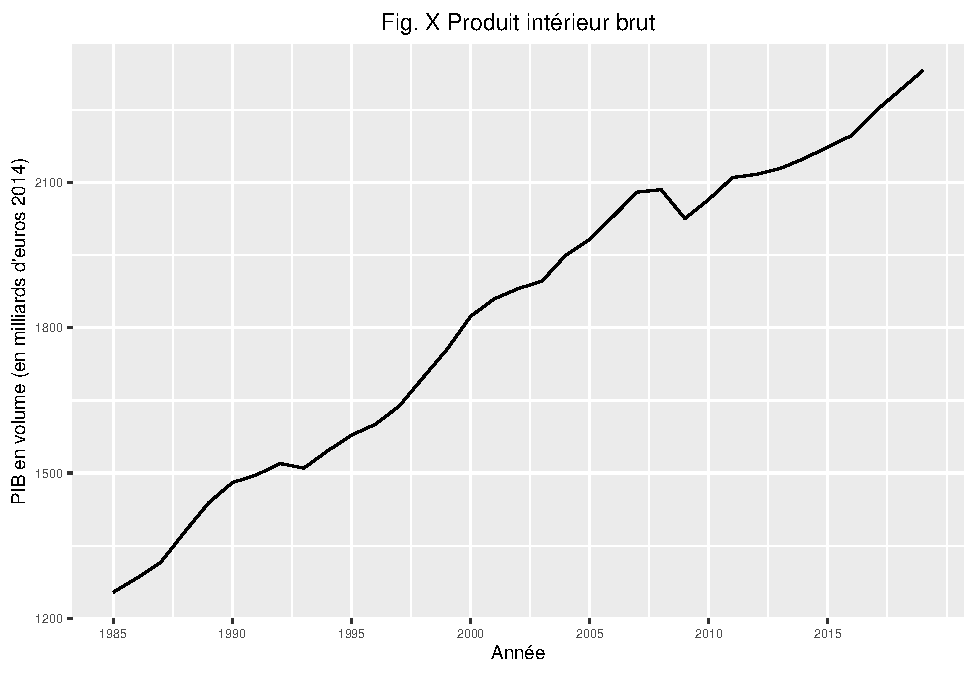
\includegraphics{Projet_econometrie_II_files/figure-latex/unnamed-chunk-4-5.pdf}

\begin{Shaded}
\begin{Highlighting}[]
\FunctionTok{plot}\NormalTok{(Qdiesel.ts, }\AttributeTok{xlab =} \StringTok{"Temps"}\NormalTok{, }\AttributeTok{ylab =} \StringTok{"Quantité de diesel consommé (tout transport confondu)"}\NormalTok{)}
\end{Highlighting}
\end{Shaded}

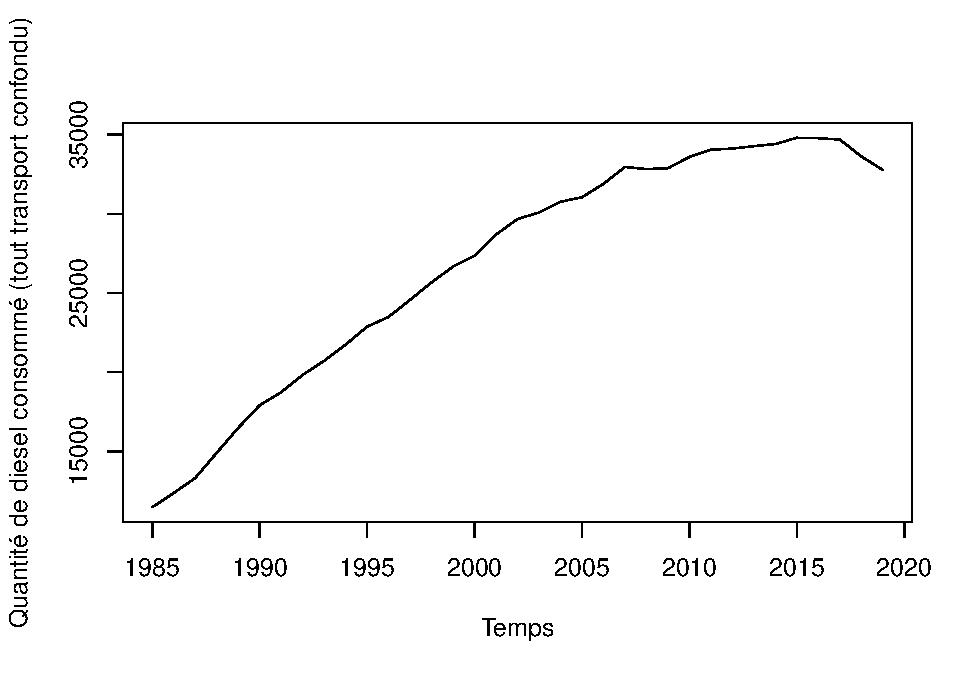
\includegraphics{Projet_econometrie_II_files/figure-latex/unnamed-chunk-4-6.pdf}

\begin{Shaded}
\begin{Highlighting}[]
\FunctionTok{plot}\NormalTok{(Qdieselcamion.ts, }\AttributeTok{xlab =} \StringTok{"Temps"}\NormalTok{, }\AttributeTok{ylab =} \StringTok{"Quantité de diesel consommé par les camions"}\NormalTok{)}
\end{Highlighting}
\end{Shaded}

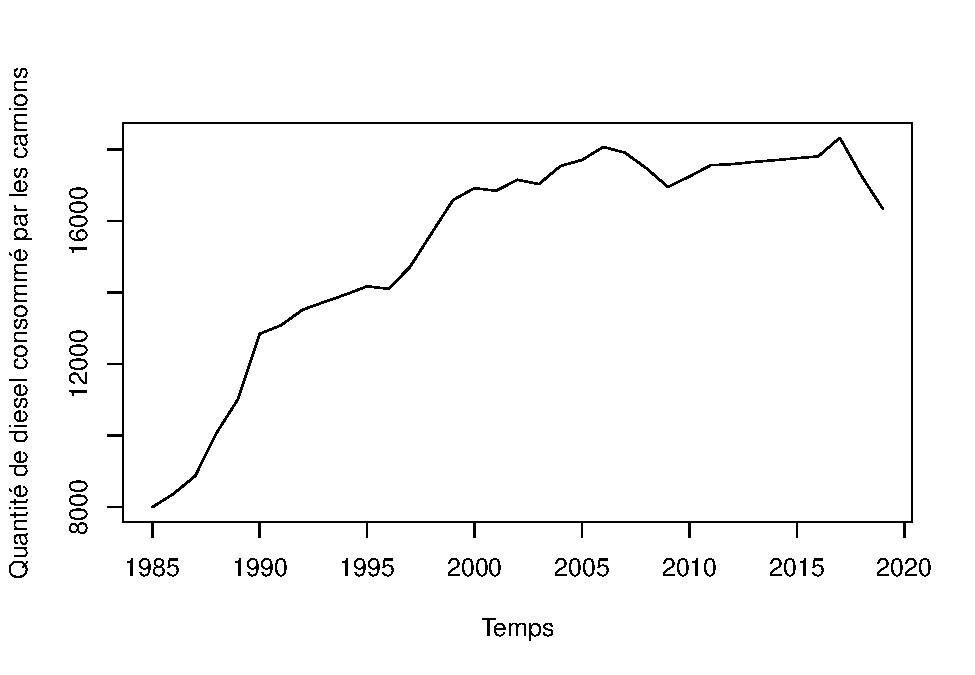
\includegraphics{Projet_econometrie_II_files/figure-latex/unnamed-chunk-4-7.pdf}

\begin{Shaded}
\begin{Highlighting}[]
\FunctionTok{plot}\NormalTok{(CPI.ts, }\AttributeTok{xlab =} \StringTok{"Temps"}\NormalTok{, }\AttributeTok{ylab =} \StringTok{"Indice de prix à la consommation"}\NormalTok{)}
\end{Highlighting}
\end{Shaded}

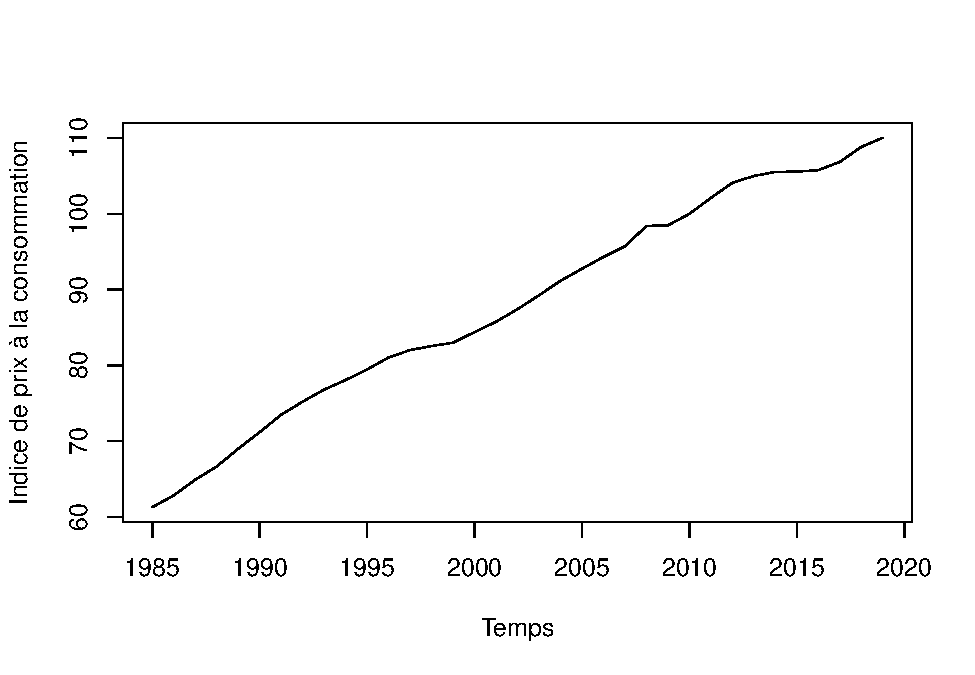
\includegraphics{Projet_econometrie_II_files/figure-latex/unnamed-chunk-4-8.pdf}

\begin{Shaded}
\begin{Highlighting}[]
\NormalTok{n}\OtherTok{=}\FunctionTok{length}\NormalTok{(Transport\_France2019}\SpecialCharTok{$}\NormalTok{Qdieselcamion)}

\NormalTok{vec }\OtherTok{\textless{}{-}} \FunctionTok{c}\NormalTok{(Transport\_France2019}\SpecialCharTok{$}\NormalTok{Pdiesel}\SpecialCharTok{/}\NormalTok{Transport\_France2019}\SpecialCharTok{$}\NormalTok{CPI,Transport\_France2019}\SpecialCharTok{$}\StringTok{"PIB en volume (en milliards d\textquotesingle{}euros 2014)"}\NormalTok{,Transport\_France2019}\SpecialCharTok{$}\NormalTok{Qtt\_Trsp\_route)}
\NormalTok{X }\OtherTok{\textless{}{-}} \FunctionTok{matrix}\NormalTok{( vec, }\AttributeTok{ncol=}\DecValTok{3}\NormalTok{) }
\NormalTok{Y}\OtherTok{=}\FunctionTok{matrix}\NormalTok{(Transport\_France2019}\SpecialCharTok{$}\NormalTok{Qdieselcamion,n,}\DecValTok{1}\NormalTok{)}
\NormalTok{q}\OtherTok{=}\FunctionTok{ncol}\NormalTok{(Y);}
\NormalTok{k}\OtherTok{=}\FunctionTok{ncol}\NormalTok{(X);}
\NormalTok{K}\OtherTok{=}\NormalTok{k}\SpecialCharTok{+}\DecValTok{1}

\NormalTok{ y}\OtherTok{=}\NormalTok{Y}
\NormalTok{ x}\OtherTok{=}\NormalTok{X}
 
\NormalTok{ nobs}\OtherTok{=}\FunctionTok{cbind}\NormalTok{(}\DecValTok{1}\SpecialCharTok{:}\NormalTok{n)}
 
\NormalTok{ OLS}\OtherTok{=}\FunctionTok{lm}\NormalTok{(}\AttributeTok{formula =}\NormalTok{ y }\SpecialCharTok{\textasciitilde{}}\NormalTok{ x)}
 
\FunctionTok{summary}\NormalTok{(OLS) }\SpecialCharTok{\%\textgreater{}\%}\NormalTok{ pander}
\end{Highlighting}
\end{Shaded}

\begin{longtable}[]{@{}
  >{\centering\arraybackslash}p{(\columnwidth - 8\tabcolsep) * \real{0.25}}
  >{\centering\arraybackslash}p{(\columnwidth - 8\tabcolsep) * \real{0.15}}
  >{\centering\arraybackslash}p{(\columnwidth - 8\tabcolsep) * \real{0.18}}
  >{\centering\arraybackslash}p{(\columnwidth - 8\tabcolsep) * \real{0.14}}
  >{\centering\arraybackslash}p{(\columnwidth - 8\tabcolsep) * \real{0.17}}@{}}
\toprule
\begin{minipage}[b]{\linewidth}\centering
~
\end{minipage} & \begin{minipage}[b]{\linewidth}\centering
Estimate
\end{minipage} & \begin{minipage}[b]{\linewidth}\centering
Std. Error
\end{minipage} & \begin{minipage}[b]{\linewidth}\centering
t value
\end{minipage} & \begin{minipage}[b]{\linewidth}\centering
Pr(\textgreater\textbar t\textbar)
\end{minipage} \\
\midrule
\endhead
\textbf{(Intercept)} & 1767 & 790.8 & 2.235 & 0.03277 \\
\textbf{x1} & -378013 & 120267 & -3.143 & 0.003667 \\
\textbf{x2} & 4.242 & 1.423 & 2.98 & 0.005559 \\
\textbf{x3} & 36.89 & 5.615 & 6.57 & 2.449e-07 \\
\bottomrule
\end{longtable}

\begin{longtable}[]{@{}
  >{\centering\arraybackslash}p{(\columnwidth - 6\tabcolsep) * \real{0.21}}
  >{\centering\arraybackslash}p{(\columnwidth - 6\tabcolsep) * \real{0.31}}
  >{\centering\arraybackslash}p{(\columnwidth - 6\tabcolsep) * \real{0.12}}
  >{\centering\arraybackslash}p{(\columnwidth - 6\tabcolsep) * \real{0.24}}@{}}
\caption{Fitting linear model: y \textasciitilde{} x}\tabularnewline
\toprule
\begin{minipage}[b]{\linewidth}\centering
Observations
\end{minipage} & \begin{minipage}[b]{\linewidth}\centering
Residual Std. Error
\end{minipage} & \begin{minipage}[b]{\linewidth}\centering
\(R^2\)
\end{minipage} & \begin{minipage}[b]{\linewidth}\centering
Adjusted \(R^2\)
\end{minipage} \\
\midrule
\endfirsthead
\toprule
\begin{minipage}[b]{\linewidth}\centering
Observations
\end{minipage} & \begin{minipage}[b]{\linewidth}\centering
Residual Std. Error
\end{minipage} & \begin{minipage}[b]{\linewidth}\centering
\(R^2\)
\end{minipage} & \begin{minipage}[b]{\linewidth}\centering
Adjusted \(R^2\)
\end{minipage} \\
\midrule
\endhead
35 & 721.2 & 0.9475 & 0.9424 \\
\bottomrule
\end{longtable}

\begin{Shaded}
\begin{Highlighting}[]
\NormalTok{ kable}
\end{Highlighting}
\end{Shaded}

\begin{verbatim}
## function (x, format, digits = getOption("digits"), row.names = NA, 
##     col.names = NA, align, caption = NULL, label = NULL, format.args = list(), 
##     escape = TRUE, ...) 
## {
##     format = kable_format(format)
##     if (!missing(align) && length(align) == 1L && !grepl("[^lcr]", 
##         align)) 
##         align = strsplit(align, "")[[1]]
##     if (inherits(x, "list")) {
##         format = kable_format_latex(format)
##         res = lapply(x, kable, format = format, digits = digits, 
##             row.names = row.names, col.names = col.names, align = align, 
##             caption = NA, format.args = format.args, escape = escape, 
##             ...)
##         return(kables(res, format, caption, label))
##     }
##     caption = kable_caption(label, caption, format)
##     if (!is.matrix(x)) 
##         x = as.data.frame(x)
##     if (identical(col.names, NA)) 
##         col.names = colnames(x)
##     m = ncol(x)
##     isn = if (is.matrix(x)) 
##         rep(is.numeric(x), m)
##     else sapply(x, is.numeric)
##     if (missing(align) || (format == "latex" && is.null(align))) 
##         align = ifelse(isn, "r", "l")
##     digits = rep(digits, length.out = m)
##     for (j in seq_len(m)) {
##         if (is_numeric(x[, j])) 
##             x[, j] = round(x[, j], digits[j])
##     }
##     if (any(isn)) {
##         if (is.matrix(x)) {
##             if (is.table(x) && length(dim(x)) == 2) 
##                 class(x) = "matrix"
##             x = format_matrix(x, format.args)
##         }
##         else x[, isn] = format_args(x[, isn], format.args)
##     }
##     if (is.na(row.names)) 
##         row.names = has_rownames(x)
##     if (!is.null(align)) 
##         align = rep(align, length.out = m)
##     if (row.names) {
##         x = cbind(` ` = rownames(x), x)
##         if (!is.null(col.names)) 
##             col.names = c(" ", col.names)
##         if (!is.null(align)) 
##             align = c("l", align)
##     }
##     n = nrow(x)
##     x = replace_na(to_character(x), is.na(x))
##     if (!is.matrix(x)) 
##         x = matrix(x, nrow = n)
##     x = trimws(x)
##     colnames(x) = col.names
##     if (format != "latex" && length(align) && !all(align %in% 
##         c("l", "r", "c"))) 
##         stop("'align' must be a character vector of possible values 'l', 'r', and 'c'")
##     attr(x, "align") = align
##     if (format == "simple" && nrow(x) == 0) 
##         format = "pipe"
##     res = do.call(paste("kable", format, sep = "_"), list(x = x, 
##         caption = caption, escape = escape, ...))
##     structure(res, format = format, class = "knitr_kable")
## }
## <bytecode: 0x000000001fcf99f0>
## <environment: namespace:knitr>
\end{verbatim}

\begin{Shaded}
\begin{Highlighting}[]
 \FunctionTok{names}\NormalTok{(OLS)}
\end{Highlighting}
\end{Shaded}

\begin{verbatim}
##  [1] "coefficients"  "residuals"     "effects"       "rank"         
##  [5] "fitted.values" "assign"        "qr"            "df.residual"  
##  [9] "xlevels"       "call"          "terms"         "model"
\end{verbatim}

\begin{Shaded}
\begin{Highlighting}[]
\NormalTok{xc }\OtherTok{=} \FunctionTok{cbind}\NormalTok{(}\DecValTok{1}\NormalTok{,x) }
\NormalTok{bhat }\OtherTok{=}\NormalTok{ OLS}\SpecialCharTok{$}\NormalTok{coefficients }
\NormalTok{yf }\OtherTok{=}\NormalTok{ xc }\SpecialCharTok{\%*\%}\NormalTok{ bhat}
\NormalTok{res }\OtherTok{=}\NormalTok{ y }\SpecialCharTok{{-}}\NormalTok{ yf}
\NormalTok{scr }\OtherTok{=} \FunctionTok{t}\NormalTok{(res) }\SpecialCharTok{\%*\%}\NormalTok{ res}


\NormalTok{d1 }\OtherTok{=} \FunctionTok{t}\NormalTok{(res) }\SpecialCharTok{\%*\%}\NormalTok{ res}
\NormalTok{d2 }\OtherTok{=}  \FunctionTok{t}\NormalTok{(res[}\DecValTok{2}\SpecialCharTok{:}\NormalTok{n]}\SpecialCharTok{{-}}\NormalTok{res[}\DecValTok{1}\SpecialCharTok{:}\NormalTok{n}\DecValTok{{-}1}\NormalTok{]) }\SpecialCharTok{\%*\%}\NormalTok{ (res[}\DecValTok{2}\SpecialCharTok{:}\NormalTok{n]}\SpecialCharTok{{-}}\NormalTok{res[}\DecValTok{1}\SpecialCharTok{:}\NormalTok{n}\DecValTok{{-}1}\NormalTok{])}
\NormalTok{dw }\OtherTok{=}\NormalTok{ d2}\SpecialCharTok{/}\NormalTok{d1}
\FunctionTok{print}\NormalTok{ (dw)}
\end{Highlighting}
\end{Shaded}

\begin{verbatim}
##           [,1]
## [1,] 0.5667082
\end{verbatim}

\begin{Shaded}
\begin{Highlighting}[]
\NormalTok{Wr }\OtherTok{\textless{}{-}} \FunctionTok{efp}\NormalTok{(y }\SpecialCharTok{\textasciitilde{}}\NormalTok{ x, }\AttributeTok{type =} \StringTok{"Rec{-}CUSUM"}\NormalTok{)}
\FunctionTok{plot}\NormalTok{(Wr)}
\end{Highlighting}
\end{Shaded}

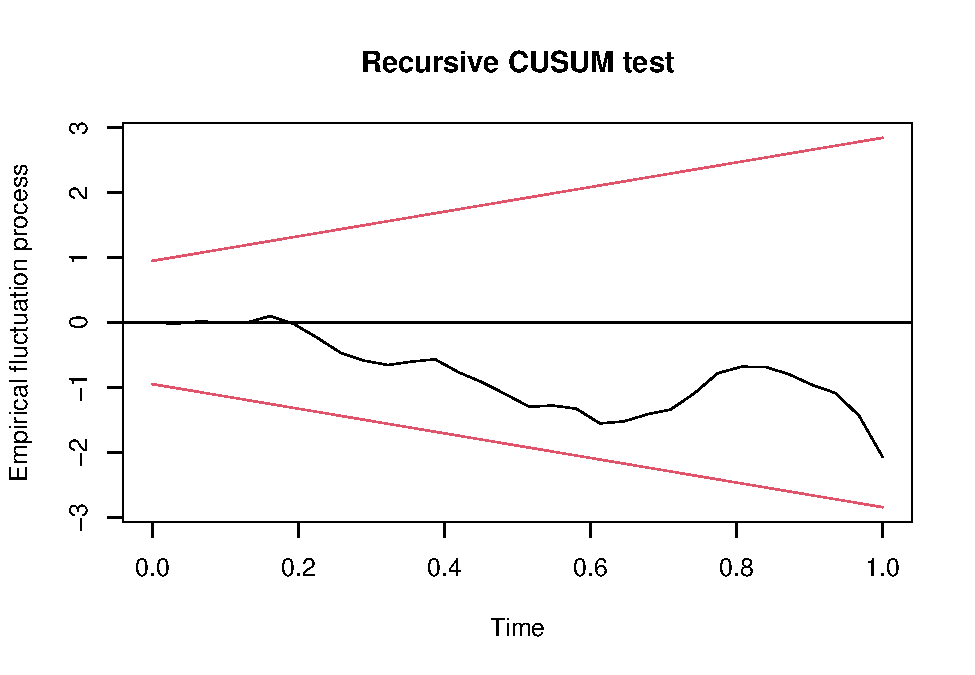
\includegraphics{Projet_econometrie_II_files/figure-latex/unnamed-chunk-6-1.pdf}

\begin{Shaded}
\begin{Highlighting}[]
\CommentTok{\#}
\CommentTok{\# Test Cusum Square}
\CommentTok{\#}
\NormalTok{rr }\OtherTok{\textless{}{-}}\NormalTok{ (}\FunctionTok{recresid}\NormalTok{(y }\SpecialCharTok{\textasciitilde{}}\NormalTok{ x))}
\NormalTok{rr }\OtherTok{\textless{}{-}}\NormalTok{ rr}\SpecialCharTok{\^{}}\DecValTok{2}
\NormalTok{cumrr }\OtherTok{\textless{}{-}} \FunctionTok{cumsum}\NormalTok{(rr)}\SpecialCharTok{/}\NormalTok{scr}
\end{Highlighting}
\end{Shaded}

\begin{verbatim}
## Warning in cumsum(rr)/scr: Le recyclage d’un tableau (array) de longueur 1 dans un calcul arithmétique vecteur-tableau est obsolète.
##   Utilisez c() ou as.vector() à la place.
\end{verbatim}

\begin{Shaded}
\begin{Highlighting}[]
\CommentTok{\#}
\CommentTok{\# Valeurs seuil de la distribution Cusum}
\CommentTok{\#}
\NormalTok{c0 }\OtherTok{=} \FloatTok{0.18915}

\NormalTok{kp2}\OtherTok{=}\NormalTok{K}\SpecialCharTok{+}\DecValTok{1}
\NormalTok{c0 }\OtherTok{=} \FloatTok{0.18915} \CommentTok{\# valeur critique de c0}

\NormalTok{t2 }\OtherTok{\textless{}{-}} \FunctionTok{ts}\NormalTok{(kp2}\SpecialCharTok{:}\NormalTok{n)}
\NormalTok{t3}\OtherTok{=}\NormalTok{t2}\DecValTok{{-}1}
\NormalTok{smin }\OtherTok{\textless{}{-}}\NormalTok{((t2}\SpecialCharTok{{-}}\NormalTok{k)}\SpecialCharTok{/}\NormalTok{(n}\SpecialCharTok{{-}}\NormalTok{k))}\SpecialCharTok{{-}}\NormalTok{c0}
\NormalTok{smax }\OtherTok{\textless{}{-}}\NormalTok{ ((t2}\SpecialCharTok{{-}}\NormalTok{k)}\SpecialCharTok{/}\NormalTok{(n}\SpecialCharTok{{-}}\NormalTok{k))}\SpecialCharTok{+}\NormalTok{c0}
\CommentTok{\#}
\NormalTok{vec2 }\OtherTok{\textless{}{-}} \FunctionTok{c}\NormalTok{(smin, cumrr, smax)}
\NormalTok{cusum2 }\OtherTok{\textless{}{-}} \FunctionTok{matrix}\NormalTok{(vec2, }\AttributeTok{ncol =} \DecValTok{3}\NormalTok{); }
\FunctionTok{matplot}\NormalTok{(}\FunctionTok{c}\NormalTok{(t3), cusum2, }\AttributeTok{type =}\StringTok{"l"}\NormalTok{)}
\end{Highlighting}
\end{Shaded}

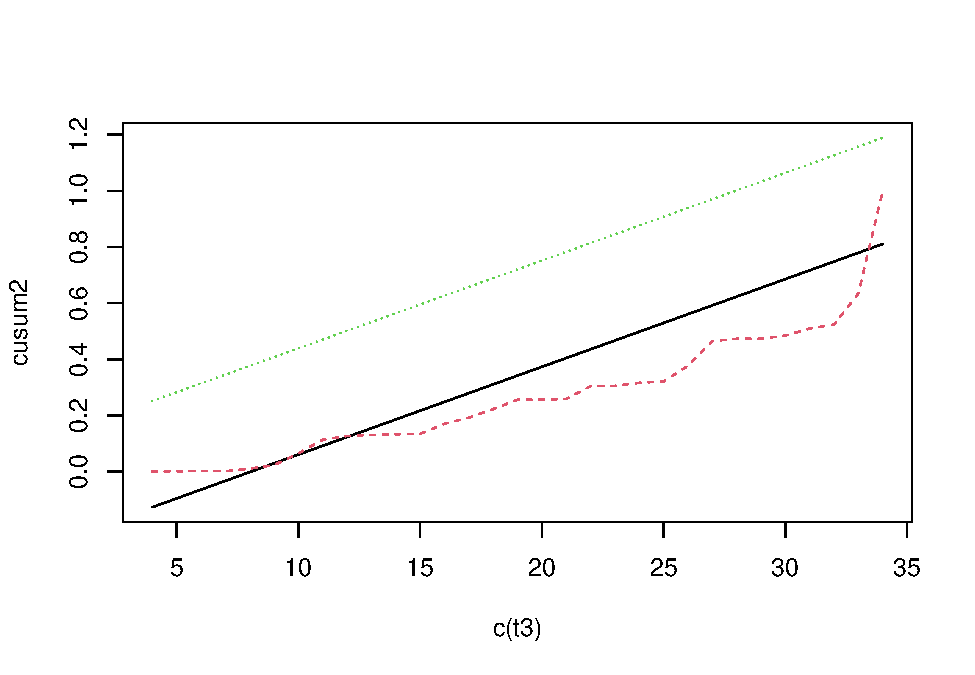
\includegraphics{Projet_econometrie_II_files/figure-latex/unnamed-chunk-6-2.pdf}

\begin{Shaded}
\begin{Highlighting}[]
\CommentTok{\#sctest(y \textasciitilde{} x, type = "Chow", point =)}
\CommentTok{\# pour R, la rupture est test?e non pas sur 1979{-}1980 mais sur 1979. }
\CommentTok{\#Sur Eviews, la rupture est test?e sur 1980/}
\ControlFlowTok{for}\NormalTok{(i }\ControlFlowTok{in} \DecValTok{9}\SpecialCharTok{:}\DecValTok{30}\NormalTok{) \{}

\FunctionTok{print}\NormalTok{(}\FunctionTok{sctest}\NormalTok{(y }\SpecialCharTok{\textasciitilde{}}\NormalTok{ x, }\AttributeTok{type =} \StringTok{"Chow"}\NormalTok{, }\AttributeTok{point =}\NormalTok{ i) )}
\NormalTok{\}}
\end{Highlighting}
\end{Shaded}

\begin{verbatim}
## 
##  Chow test
## 
## data:  y ~ x
## F = 4.6272, p-value = 0.005642
## 
## 
##  Chow test
## 
## data:  y ~ x
## F = 4.6428, p-value = 0.005547
## 
## 
##  Chow test
## 
## data:  y ~ x
## F = 4.6513, p-value = 0.005497
## 
## 
##  Chow test
## 
## data:  y ~ x
## F = 5.796, p-value = 0.00168
## 
## 
##  Chow test
## 
## data:  y ~ x
## F = 8.5115, p-value = 0.0001406
## 
## 
##  Chow test
## 
## data:  y ~ x
## F = 10.764, p-value = 2.389e-05
## 
## 
##  Chow test
## 
## data:  y ~ x
## F = 11.173, p-value = 1.772e-05
## 
## 
##  Chow test
## 
## data:  y ~ x
## F = 11.398, p-value = 1.507e-05
## 
## 
##  Chow test
## 
## data:  y ~ x
## F = 10.585, p-value = 2.728e-05
## 
## 
##  Chow test
## 
## data:  y ~ x
## F = 10.003, p-value = 4.242e-05
## 
## 
##  Chow test
## 
## data:  y ~ x
## F = 9.932, p-value = 4.48e-05
## 
## 
##  Chow test
## 
## data:  y ~ x
## F = 8.8977, p-value = 0.0001021
## 
## 
##  Chow test
## 
## data:  y ~ x
## F = 8.902, p-value = 0.0001017
## 
## 
##  Chow test
## 
## data:  y ~ x
## F = 9.1596, p-value = 8.247e-05
## 
## 
##  Chow test
## 
## data:  y ~ x
## F = 8.2241, p-value = 0.0001793
## 
## 
##  Chow test
## 
## data:  y ~ x
## F = 8.8558, p-value = 0.0001056
## 
## 
##  Chow test
## 
## data:  y ~ x
## F = 9.8364, p-value = 4.825e-05
## 
## 
##  Chow test
## 
## data:  y ~ x
## F = 11.003, p-value = 2.004e-05
## 
## 
##  Chow test
## 
## data:  y ~ x
## F = 9.5052, p-value = 6.256e-05
## 
## 
##  Chow test
## 
## data:  y ~ x
## F = 7.0616, p-value = 0.0005013
## 
## 
##  Chow test
## 
## data:  y ~ x
## F = 6.9945, p-value = 0.0005331
## 
## 
##  Chow test
## 
## data:  y ~ x
## F = 7.5019, p-value = 0.0003366
\end{verbatim}

\begin{Shaded}
\begin{Highlighting}[]
\NormalTok{n}\OtherTok{=}\FunctionTok{length}\NormalTok{(Transport\_France2019}\SpecialCharTok{$}\NormalTok{Qdieselcamion)}

\NormalTok{P1 }\OtherTok{\textless{}{-}} \FunctionTok{replicate}\NormalTok{(}\DecValTok{35}\NormalTok{, }\DecValTok{0}\NormalTok{)}
\NormalTok{P1[}\DecValTok{1}\SpecialCharTok{:}\DecValTok{16}\NormalTok{] }\OtherTok{\textless{}{-}}\NormalTok{  Transport\_France2019}\SpecialCharTok{$}\NormalTok{Pdiesel[}\DecValTok{1}\SpecialCharTok{:}\DecValTok{16}\NormalTok{]}\SpecialCharTok{/}\NormalTok{Transport\_France2019}\SpecialCharTok{$}\NormalTok{CPI[}\DecValTok{1}\SpecialCharTok{:}\DecValTok{16}\NormalTok{]}

\NormalTok{P2 }\OtherTok{\textless{}{-}} \FunctionTok{replicate}\NormalTok{(}\DecValTok{35}\NormalTok{, }\DecValTok{0}\NormalTok{)}
\NormalTok{P2[}\DecValTok{17}\SpecialCharTok{:}\DecValTok{35}\NormalTok{] }\OtherTok{\textless{}{-}}\NormalTok{  Transport\_France2019}\SpecialCharTok{$}\NormalTok{Pdiesel[}\DecValTok{17}\SpecialCharTok{:}\DecValTok{35}\NormalTok{]}\SpecialCharTok{/}\NormalTok{Transport\_France2019}\SpecialCharTok{$}\NormalTok{CPI[}\DecValTok{17}\SpecialCharTok{:}\DecValTok{35}\NormalTok{]}

\NormalTok{vec }\OtherTok{\textless{}{-}} \FunctionTok{c}\NormalTok{(P1,P2, Transport\_France2019}\SpecialCharTok{$}\StringTok{"PIB en volume (en milliards d\textquotesingle{}euros 2014)"}\NormalTok{,Transport\_France2019}\SpecialCharTok{$}\NormalTok{Qtt\_Trsp\_route)}
\NormalTok{X }\OtherTok{\textless{}{-}} \FunctionTok{matrix}\NormalTok{( vec, }\AttributeTok{ncol=}\DecValTok{4}\NormalTok{) }
\NormalTok{Y}\OtherTok{=}\FunctionTok{matrix}\NormalTok{(Transport\_France2019}\SpecialCharTok{$}\NormalTok{Qdieselcamion,n,}\DecValTok{1}\NormalTok{)}
\NormalTok{q}\OtherTok{=}\FunctionTok{ncol}\NormalTok{(Y);}
\NormalTok{k}\OtherTok{=}\FunctionTok{ncol}\NormalTok{(X);}
\NormalTok{K}\OtherTok{=}\NormalTok{k}\SpecialCharTok{+}\DecValTok{1}

\NormalTok{ y}\OtherTok{=}\NormalTok{Y}
\NormalTok{ x}\OtherTok{=}\NormalTok{X}
 
\NormalTok{ nobs}\OtherTok{=}\FunctionTok{cbind}\NormalTok{(}\DecValTok{1}\SpecialCharTok{:}\NormalTok{n)}
 
\NormalTok{ OLS}\OtherTok{=}\FunctionTok{lm}\NormalTok{(}\AttributeTok{formula =}\NormalTok{ y }\SpecialCharTok{\textasciitilde{}}\NormalTok{ x)}
 
 \FunctionTok{summary}\NormalTok{(OLS)}
\end{Highlighting}
\end{Shaded}

\begin{verbatim}
## 
## Call:
## lm(formula = y ~ x)
## 
## Residuals:
##      Min       1Q   Median       3Q      Max 
## -2393.64  -264.17    46.23   364.36  1468.79 
## 
## Coefficients:
##               Estimate Std. Error t value Pr(>|t|)    
## (Intercept)  1.174e+02  1.670e+03   0.070  0.94445    
## x1          -2.946e+05  1.410e+05  -2.089  0.04528 *  
## x2          -3.651e+05  1.203e+05  -3.034  0.00495 ** 
## x3           4.871e+00  1.525e+00   3.195  0.00328 ** 
## x4           3.735e+01  5.607e+00   6.661 2.23e-07 ***
## ---
## Signif. codes:  0 '***' 0.001 '**' 0.01 '*' 0.05 '.' 0.1 ' ' 1
## 
## Residual standard error: 718.3 on 30 degrees of freedom
## Multiple R-squared:  0.9496, Adjusted R-squared:  0.9429 
## F-statistic: 141.4 on 4 and 30 DF,  p-value: < 2.2e-16
\end{verbatim}

\begin{Shaded}
\begin{Highlighting}[]
 \FunctionTok{names}\NormalTok{(OLS)}
\end{Highlighting}
\end{Shaded}

\begin{verbatim}
##  [1] "coefficients"  "residuals"     "effects"       "rank"         
##  [5] "fitted.values" "assign"        "qr"            "df.residual"  
##  [9] "xlevels"       "call"          "terms"         "model"
\end{verbatim}

\begin{Shaded}
\begin{Highlighting}[]
\NormalTok{xc }\OtherTok{=} \FunctionTok{cbind}\NormalTok{(}\DecValTok{1}\NormalTok{,x) }
\NormalTok{bhat }\OtherTok{=}\NormalTok{ OLS}\SpecialCharTok{$}\NormalTok{coefficients }
\NormalTok{yf }\OtherTok{=}\NormalTok{ xc }\SpecialCharTok{\%*\%}\NormalTok{ bhat}
\NormalTok{res }\OtherTok{=}\NormalTok{ y }\SpecialCharTok{{-}}\NormalTok{ yf}
\NormalTok{scr }\OtherTok{=} \FunctionTok{t}\NormalTok{(res) }\SpecialCharTok{\%*\%}\NormalTok{ res}


\NormalTok{d1 }\OtherTok{=} \FunctionTok{t}\NormalTok{(res) }\SpecialCharTok{\%*\%}\NormalTok{ res}
\NormalTok{d2 }\OtherTok{=}  \FunctionTok{t}\NormalTok{(res[}\DecValTok{2}\SpecialCharTok{:}\NormalTok{n]}\SpecialCharTok{{-}}\NormalTok{res[}\DecValTok{1}\SpecialCharTok{:}\NormalTok{n}\DecValTok{{-}1}\NormalTok{]) }\SpecialCharTok{\%*\%}\NormalTok{ (res[}\DecValTok{2}\SpecialCharTok{:}\NormalTok{n]}\SpecialCharTok{{-}}\NormalTok{res[}\DecValTok{1}\SpecialCharTok{:}\NormalTok{n}\DecValTok{{-}1}\NormalTok{])}
\NormalTok{dw }\OtherTok{=}\NormalTok{ d2}\SpecialCharTok{/}\NormalTok{d1}
\FunctionTok{print}\NormalTok{ (dw)}
\end{Highlighting}
\end{Shaded}

\begin{verbatim}
##           [,1]
## [1,] 0.5232029
\end{verbatim}

\printbibliography

\end{document}
